%%%%%%%%%%%%%%%%%%%%%%%%%%%%%%%%%%%%%%%%%
% Beamer Presentation
% LaTeX Template
% Version 1.0 (10/11/12)
%
% This template has been downloaded from:
% http://www.LaTeXTemplates.com
%
% License:
% CC BY-NC-SA 3.0 (http://creativecommons.org/licenses/by-nc-sa/3.0/)
%
%%%%%%%%%%%%%%%%%%%%%%%%%%%%%%%%%%%%%%%%%

%----------------------------------------------------------------------------------------
%	PACKAGES AND THEMES
%----------------------------------------------------------------------------------------

\documentclass{beamer}

\mode<presentation> {

% The Beamer class comes with a number of default slide themes
% which change the colors and layouts of slides. Below this is a list
% of all the themes, uncomment each in turn to see what they look like.

%\usetheme{default}
%\usetheme{AnnArbor}
%\usetheme{Antibes}
%\usetheme{Bergen}
%\usetheme{Berkeley}
%\usetheme{Berlin}
%\usetheme{Boadilla}
%\usetheme{CambridgeUS}
%\usetheme{Copenhagen}
%\usetheme{Darmstadt}
%\usetheme{Dresden}
%\usetheme{Frankfurt}
%\usetheme{Goettingen}
%\usetheme{Hannover}
%\usetheme{Ilmenau}
%\usetheme{JuanLesPins}
%\usetheme{Luebeck}
\usetheme{Madrid}
%\usetheme{Malmoe}
%\usetheme{Marburg}
%\usetheme{Montpellier}
%\usetheme{PaloAlto}
%\usetheme{Pittsburgh}
%\usetheme{Rochester}
%\usetheme{Singapore}
%\usetheme{Szeged}
%\usetheme{Warsaw}

% As well as themes, the Beamer class has a number of color themes
% for any slide theme. Uncomment each of these in turn to see how it
% changes the colors of your current slide theme.

%\usecolortheme{albatross}
%\usecolortheme{beaver}
%\usecolortheme{beetle}
%\usecolortheme{crane}
%\usecolortheme{dolphin}
%\usecolortheme{dove}
%\usecolortheme{fly}
%\usecolortheme{lily}
%\usecolortheme{orchid}
%\usecolortheme{rose}
%\usecolortheme{seagull}
%\usecolortheme{seahorse}
%\usecolortheme{whale}
%\usecolortheme{wolverine}

%\setbeamertemplate{footline} % To remove the footer line in all slides uncomment this line
%\setbeamertemplate{footline}[page number] % To replace the footer line in all slides with a simple slide count uncomment this line

\setbeamertemplate{navigation symbols}{} % To remove the navigation symbols from the bottom of all slides uncomment this line
}

\usepackage{graphicx} % Allows including images
\usepackage{booktabs} % Allows the use of \toprule, \midrule and \bottomrule in tables
\usepackage{graphicx}

%----------------------------------------------------------------------------------------
%	TITLE PAGE
%----------------------------------------------------------------------------------------

\title[Evolving Part-DNA Substructures]{The Automated Modeling and Optimization of Part DNA Substructures Employing Evolutionary Computation} % The short title appears at the bottom of every slide, the full title is only on the title page

\author{Daniel Tauritz, Bailey Eversmeyer} % Your name
\institute[S\&T] % Your institution as it will appear on the bottom of every slide, may be shorthand to save space
{
Missouri University of Science and Technology \\ % Your institution for the title page
Department of Computer Science

\medskip
\textit{tauritzd@mst.edu, rbe62d@mst.edu} % Your email address
}
\date{\today} % Date, can be changed to a custom date

\begin{document}

\begin{frame}
\titlepage % Print the title page as the first slide
\end{frame}

\begin{frame}
\frametitle{Overview} % Table of contents slide, comment this block out to remove it
\tableofcontents % Throughout your presentation, if you choose to use \section{} and \subsection{} commands, these will automatically be printed on this slide as an overview of your presentation
\end{frame}

\section{Part-DNA}

\begin{frame}
\frametitle{Part-DNA Overview}
Goals:
\begin{itemize}
\item Model and map the flow of goods and components

through a system\pause
\item Track the changes to components over time\pause
\item Help identify relationships between components\pause
\item Makes analyzing the system easier
\end{itemize}
\end{frame}

\begin{frame}
\frametitle{How We Fit into the Part-DNA Model}
\begin{enumerate}
\item Choose a substructure of the Part-DNA Model\pause
\item Modeling the substructure (GP)
%\item Optimize input combinations (MOEA)
%\item Gather data on input-output component transformations\pause
%\item Model the transformations of components\pause
%\item Gather data on possible input components\pause
%\item Test new input combinations to map Pareto Trade-Off surface
\end{enumerate}
\end{frame}

\begin{frame}
\frametitle{Modeling the Substructure}
\begin{enumerate}
%\item Choose a substructure of the Part-DNA Model\pause
%\item Modeling the substructure (GP)\pause
%\item Optimize input combinations (MOEA)
\item Map the layout into a well-defined ordering
%\item Gather data on input-output component transformations\pause
%\item Model the transformations of components
%\item Gather data on possible input components\pause
%\item Test new input combinations to map Pareto Trade-Off surface
\end{enumerate}
\end{frame}

\begin{frame}
\frametitle{Our Model Concept}
\begin{figure}
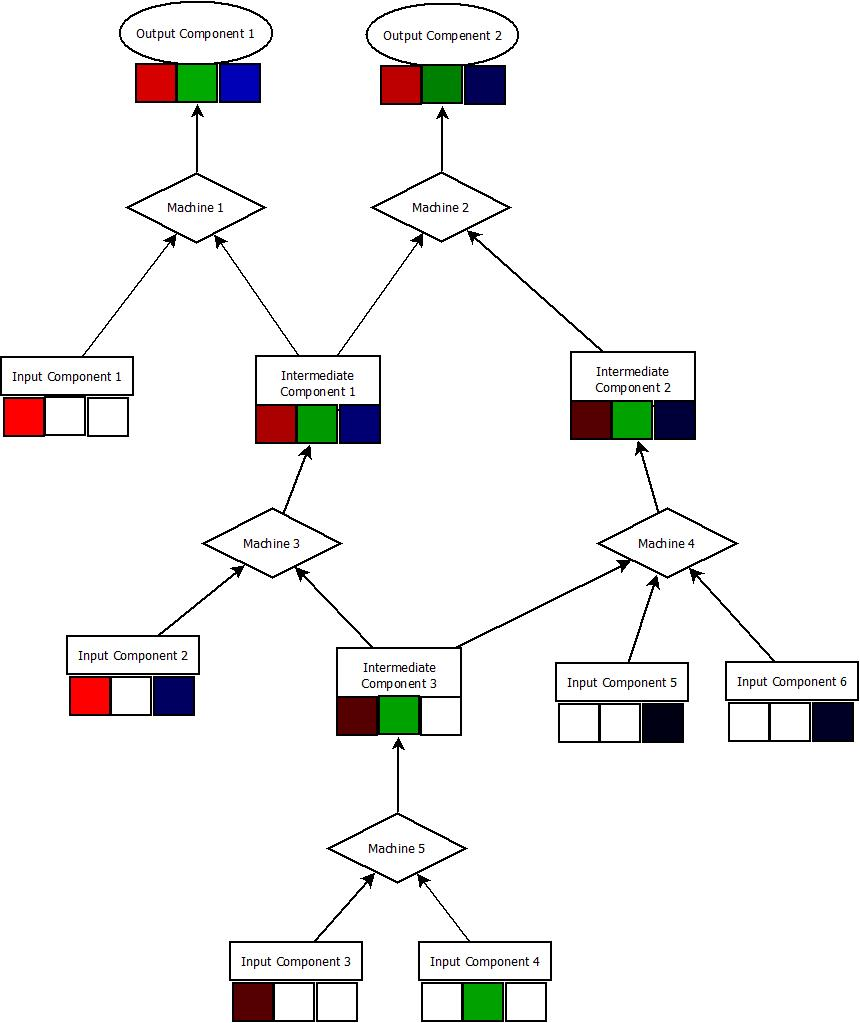
\includegraphics[width=0.5\linewidth]{BaseModel.jpeg}
\end{figure}
\end{frame}

\begin{frame}
\frametitle{Modeling the Substructure}
\begin{enumerate}
%\item Choose a substructure of the Part-DNA Model\pause
%\item Modeling the substructure (GP)\pause
%\item Optimize input combinations (MOEA)
\item Map the layout into a well-defined ordering
\item Gather data on input-output component transformations\pause
\item Model the transformations of components
%\item Gather data on possible input components\pause
%\item Test new input combinations to map Pareto Trade-Off surface
\end{enumerate}
\end{frame}

\begin{frame}
\frametitle{How We Fit into the Part-DNA Model}
\begin{enumerate}
\item Choose a substructure of the Part-DNA Model
\item Modeling the substructure (GP)\pause
\item Optimize input combinations (MOEA)
%\item Gather data on input-output component transformations\pause
%\item Model the transformations of components\pause
%\item Gather data on possible input components\pause
%\item Test new input combinations to map Pareto Trade-Off surface
\end{enumerate}
\end{frame}

\begin{frame}
\frametitle{Optimizing the Substructure}
With the model in hand:
\begin{enumerate}
%\item Choose a substructure of the Part-DNA Model\pause
%\item Modeling the substructure (GP)\pause
%\item Optimize input combinations (MOEA)
%\item Gather data on input-output component transformations\pause
%\item Model the transformations of components
\item Gather data on possible input components\pause
\item Test new input combinations to map Pareto Trade-Off surface
\end{enumerate}
\end{frame}

\section{Evolutionary Computation Strategies}

\begin{frame}
\frametitle{Evolutionary Algorithms (EAs)}
\begin{itemize}
\item EAs are stochastic, population-based local search algorithms

inspired by neo-Darwinian Evolution Theory\pause
\item Work by generating solutions, and testing fitness\pause
\item Explore search space through recombination and mutation\pause
\item Best population members chosen via Survival-of-the-fittest\pause
\item Individual \textbf{A} is better than individual \textbf{B} if \textbf{A} has a higher

fitness than \textbf{B}
\end{itemize}
\end{frame}

\subsection{Genetic Programming}

\begin{frame}[fragile]
\frametitle{Genetic Programming (GP)}
\begin{itemize}
\item Variable-size hierarchical representation vs fixed-size linear

for EAs\pause
\item Generally a tree-like structure that can model functions:\pause
\begin{equation}
Y = X^2 + sin(X*\pi)
\end{equation}
\end{itemize}
\begin{figure}
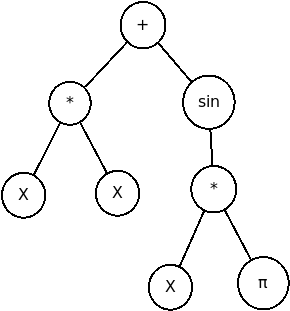
\includegraphics[width=0.3\linewidth]{functionmodel.png}
\end{figure}
\end{frame}

\subsection{Multi-Objective Evolutionary Algorithms}

\begin{frame}
\frametitle{Multi-Objective EAs (MOEAs)}
\begin{itemize}
\item Extension of regular EAs which maps multiple objective

values to single fitness\pause
\item Objectives usually conflict\pause
\item Uses \textit{Dominance} in place of fitness\pause
\item Individual \textbf{A} dominates individual \textbf{B} iff:\pause
	\begin{itemize}		
	\item \textbf{A} is no worse than \textbf{B} in all objectives\pause
	\item \textbf{A} is strictly better than \textbf{B} in at least one objective
	\end{itemize}
\end{itemize}
\end{frame}

\begin{frame}[fragile]
\frametitle{MOEA Dominance}
\begin{itemize}
\item \textbf{A} \textit{dominates} \textbf{B}
	\begin{itemize}
	\item \textbf{A:} \verb|Accuracy 60%, Affordability 2|
	\item \textbf{B:} \verb|Accuracy 50%, Affordability 2|\pause
	\end{itemize}
\item \textbf{A} does \textit{not dominate} \textbf{B}
	\begin{itemize}
	\item \textbf{A:} \verb|Accuracy 60%, Affordability 1|
	\item \textbf{B:} \verb|Accuracy 50%, Affordability 2|
	\end{itemize}
\end{itemize}
\end{frame}

\section{Application of EC Strategies}

\subsection{GP Modeling}
\begin{frame}
\frametitle{GP Section}
\begin{figure}
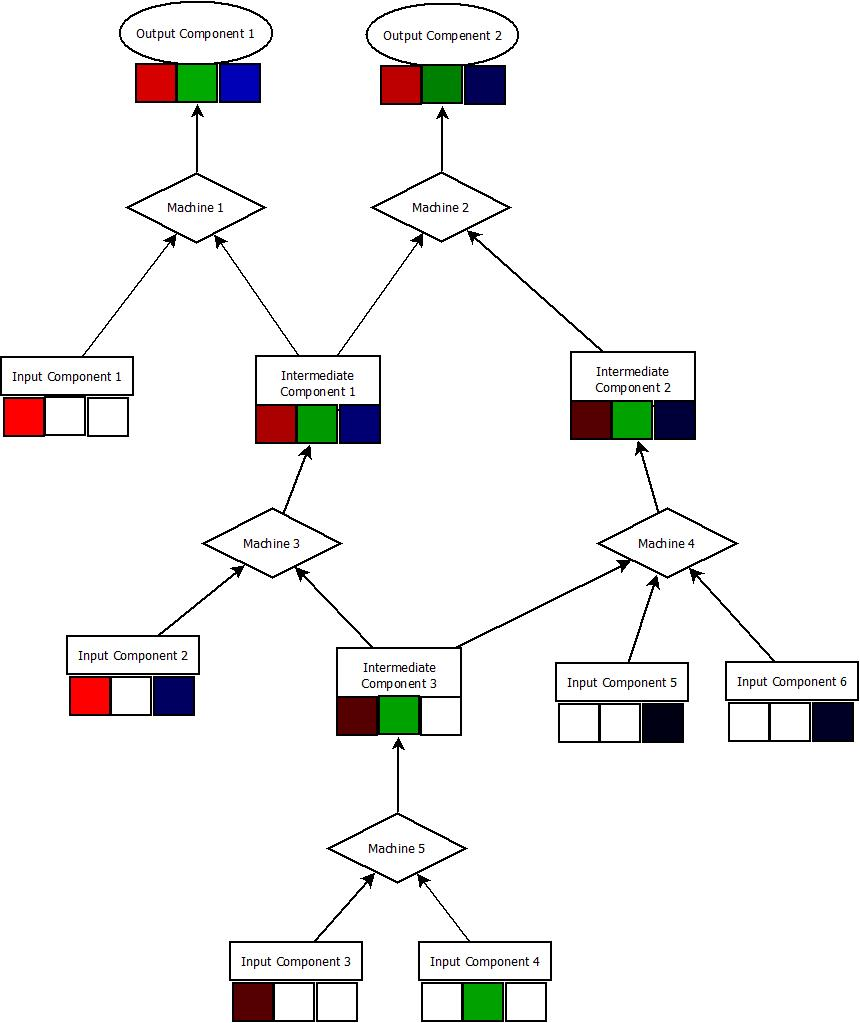
\includegraphics[width=0.5\linewidth]{BaseModel.jpeg}
\end{figure}
\end{frame}

\begin{frame}
\frametitle{GP Section}
\begin{figure}
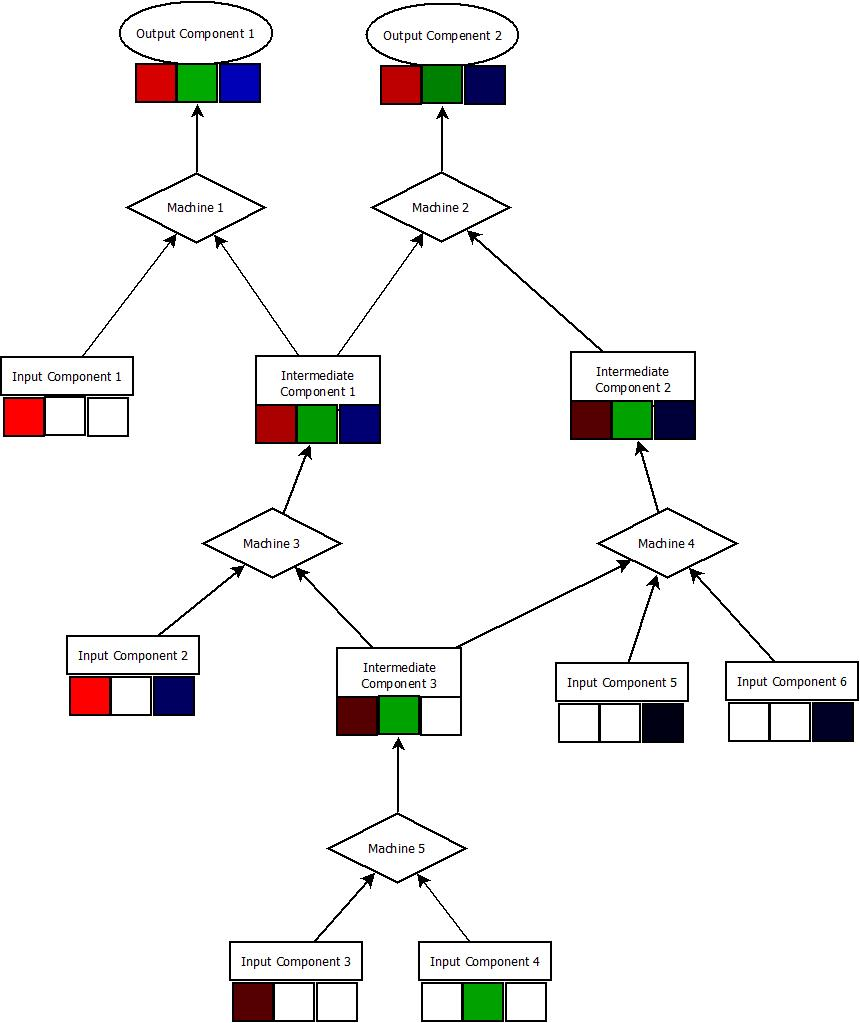
\includegraphics[width=0.5\linewidth, trim={6cm 0 8.1cm 17.1cm},clip]{BaseModel.jpeg}
\end{figure}
\end{frame}

\begin{frame}
\frametitle{GP Process}
Given a dataset of input-output combinations

For each output attribute:
\begin{itemize}
\item Generate population of randomized functions from the

input domain\pause
\item Assign fitness value based on error across the dataset\pause
\item Explore the function domain through recombination and

mutation of functions
\end{itemize}
Repeat for each transformation object
\end{frame}

\subsection{MOEA Optimization}
\begin{frame}
\frametitle{MOEA Section}
With the modeled functions in hand, we apply our MOEA to the

whole process to optimize for the output parameters
\begin{figure}
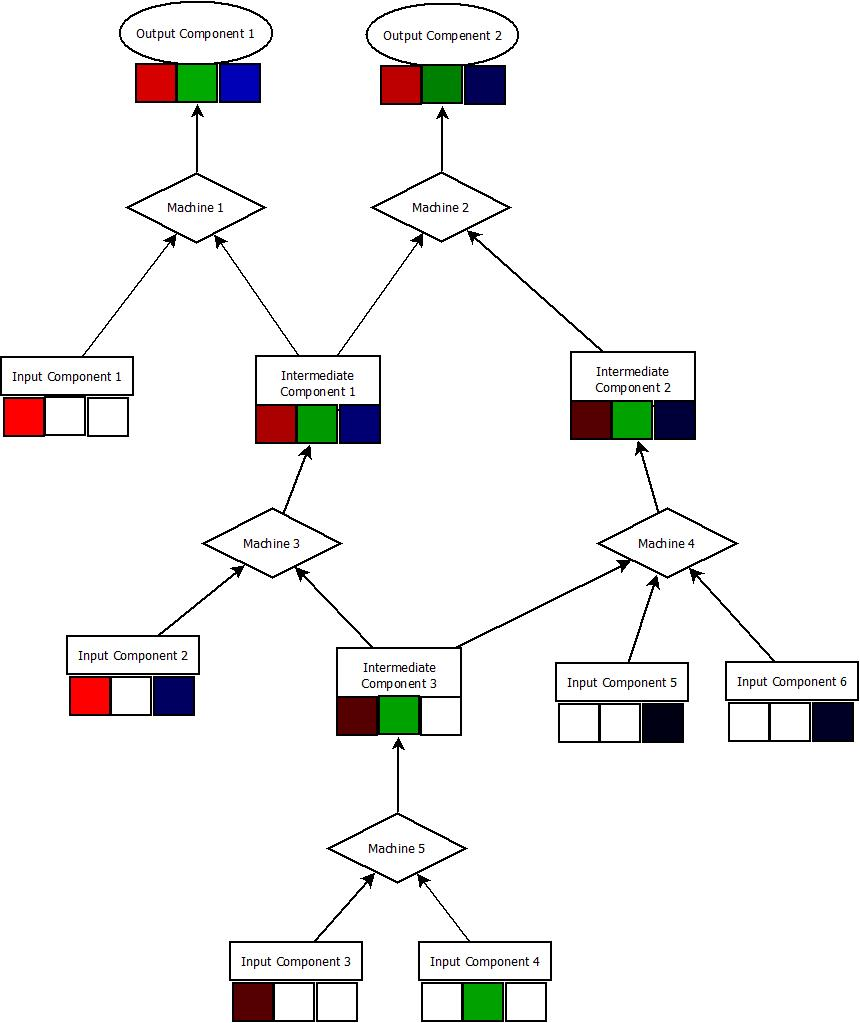
\includegraphics[width=0.4\linewidth]{BaseModel.jpeg}
\end{figure}
\end{frame}

\begin{frame}
\frametitle{MOEA Process}
Given a dataset of possible inputs and desired outputs:
\begin{itemize}
\item Generate population of randomly chosen inputs\pause
\item Simulate the system with each input combination\pause
\item Assign fitness values for Accuracy and Affordability\pause
\item Rate solutions based on their Pareto score\pause
\item Explore the input combination domain through recombination

and mutation of solutions
\end{itemize}
End with a selection of Pareto Optimal solutions, and associated

trade-off information.
\end{frame}

\begin{frame}
\frametitle{Example Pareto Front over Time}
\begin{figure}
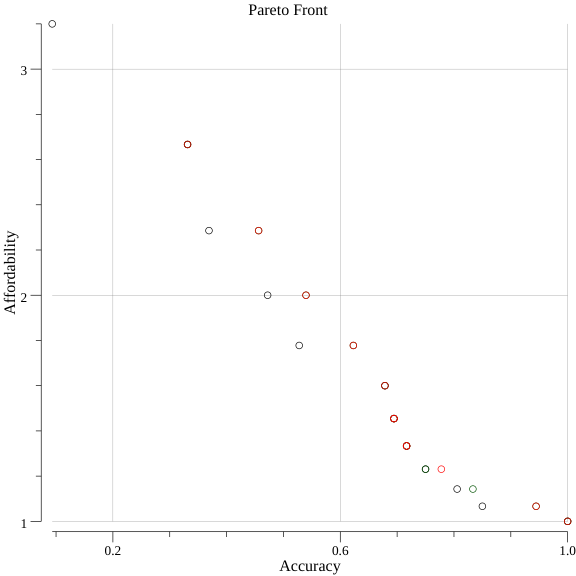
\includegraphics[width=0.6\linewidth]{points.png}
\end{figure}
\end{frame}

\section{Future Work}
\begin{frame}
\frametitle{Future of the Project}
\begin{itemize}
\item Realistic datasets, both transformation machines and

full substructure simulation\pause
\item Possibility for optimizing full substructure layout/ordering
\end{itemize}
\end{frame}

\begin{frame}
\Huge{\centerline{Questions?}}
\end{frame}

\begin{frame}[fragile]
\frametitle{References}
\begin{itemize}
\item Dr. Tauritz's Intro to EA class slides 
	\begin{itemize}	
	\item \verb|http://web.mst.edu/~tauritzd/courses/ec/|
	\end{itemize}
\end{itemize}
\end{frame}

\end{document}